\chapter{Introduction}\label{chapter:introduction}
According to the Lawson criterion, for nuclear fusion to occur, the product of particle density $n$, temperature $T$, and confinement time $\tau$ must be above a critical value.
\begin{align} % Lawson Criterion
	n\,T\,\tau_E \geq 3\times 10^{21}~\frac{\text{keV}\cdot\text{s}}{\text{m}^3}
\end{align}
In this expression, the confinement time is generally regarded to be the term that limits progress in development of fusion, as it has been the most difficult to increase.
Currently, no experiment has achieved this criterion, also referred to as ``ignition.''

In 1982, a new neutral-beam injection heating system was install in the ASDEX tokamak, which pushed the device into a new realm of operation.
An increased level of energy confinement time was achieved, measured to be a factor of 2 or more than what was expected.
This state of operation was coined the high-confinement (H--) mode, and is now considered necessary for the future of nuclear fusion as an energy source \cite{arnoux_how_2009, wagner_development_1984}.
With this new level of energy confinement, the community got one step closer to economic fusion power plants.
The details of this transition, however, are still not fully understood.

\section{L-- and H--Mode in Tokamak Plasmas}\label{sec:L_H_mode}
\subsection{Characteristics}\label{ssec:characteristics}
Transport of particles and energy in tokamaks has been discovered to be significantly dominated by anomalous transport.
This form of transport is generally assumed to be generated by turbulence, which are driven by micro-instabilities.
Low-confinement mode, referred to as L--mode, is dominated by this transport at the edge.
The formation of H--mode is due to the suppression of this turbulent transport.
This mode is therefore categorized as having a transport barrier, with particle and heat diffusivity significantly less than in L--mode at the plasma edge.
This results in an increase to the confinement time $\tau_E$.

\begin{figure}[tb] % L--H-modes compare
\begin{minipage}{0.49\linewidth}
	\centering
	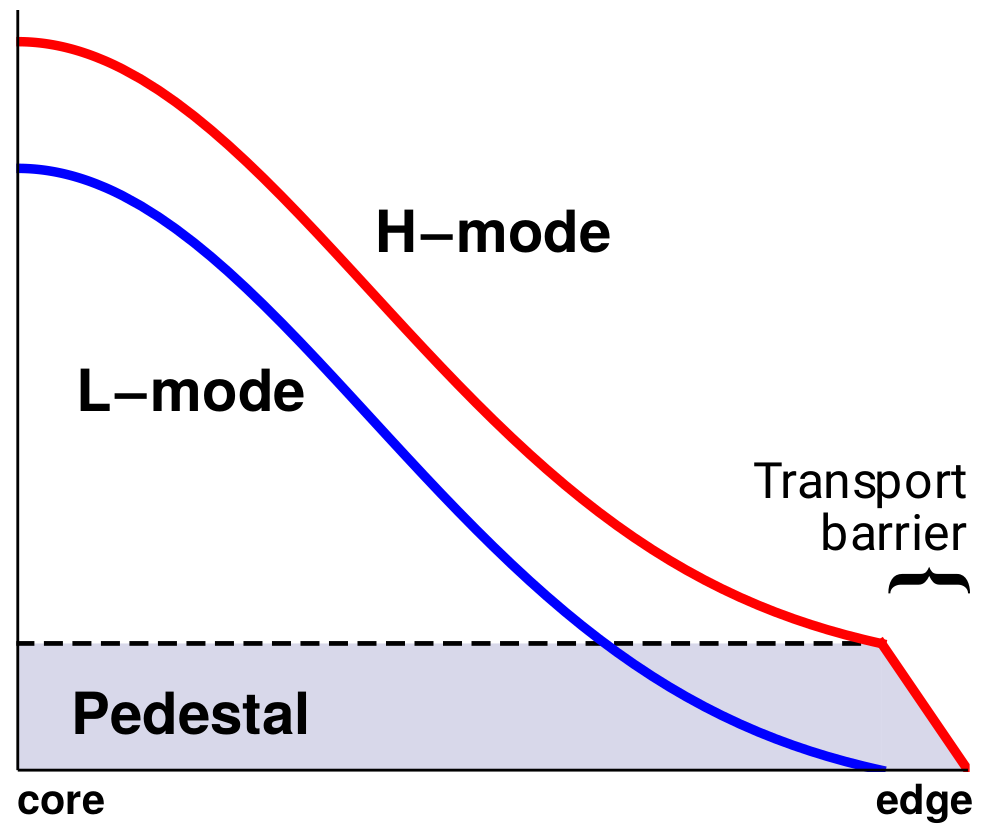
\includegraphics[width=0.8\textwidth]{../Graphics/L-mode_H-mode_compare.png}
\end{minipage}
\hfill
\begin{minipage}{0.49\linewidth}
	\caption{A comparison of the radial pressure profiles of L--mode and H--mode.
	The profile of H--mode can be thought of as on a ``pedestal,'' in which the pressure profile is increase in the core.
	This is due to the transport barrier that is formed at the edge \cite{weymiens_bifurcation_2014}.}
	\label{fig:L-mode_H-mode_compare}
\end{minipage}
\end{figure}

One of the properties of H--mode is its significantly-raised pressure profile compared to that of L--mode, and is said to sit on a ``pedestal.''
Accordingly, there is a steep gradient in the pressure at the edge of the plasma, shown and compared to L--mode in Figure~\ref{fig:L-mode_H-mode_compare} \cite{weymiens_bifurcation_2014}.
The increase in confinement allows for an increased temperature in the core.

In addition, hysteresis is present between the modes, in which the threshold power for the transition between the two modes is based on the current mode.
More information on this is in Section~\ref{ssec:hysteresis}.

\subsection{Transition}\label{ssec:transition}
The key feature that determines a divertor tokamak's operational mode is the amount of external heating power.
Limiter tokamaks are relegated to stay in L--mode, as H--mode is an exclusive operating mode of tokamaks with divertors.
The transition has been observed to occur in one of three manners: sharp, smooth, and oscillatory.
These observations therefore suggest that, mathematically, the transition comes as a result of the bifurcation of the plasma state.
The manner of the transition is based primarily on the density of the plasma, with lower density resulting in the smooth transition \cite{sauter_l--_2012}.
As mentioned previously, hysteresis can be present between the modes, occurring in accordance with a sharp transition.

The exact physical mechanism (rather than engineering parameter) that induces the transition to occur is still unknown \cite{itoh_structural_2016}.
However, the dynamics observed in the transition can be identified to be particular bifurcations, suggesting the dynamical equations \cite{weymiens_bifurcation_2012}.
Bifurcation theory is the area of mathematics that describes the changes in qualitative solutions of a system, of which the L--H transition can be described.
The details of this theory is covered in Section~\ref{sec:bif_theory}.

\subsection{Dynamics}\label{ssec:dynamics}
The suppression of turbulent transport is accepted to be caused by sheared plasma flow.
Shear stress tears apart turbulence structures, such as eddies, transferring the energy to larger structures.
A radial electric field causes an $\mathbf{E}\times\mathbf{B}$-flow, which its gradient is able to sustain the sheared flow.
Experiments done at the TEXTOR tokamak were able to artificially induce the transition to H--mode by means of a biased electrode \cite{weynants_confinement_1992}.

A few models have been developed to investigate the dynamics of H--mode and the transition.
Investigated in this project is two which simulate the radial electric field, the first originally conceived by Zohm \cite{zohm_dynamic_1994} and further developed \cite{paquay_studying_2012} \cite{weymiens_bifurcation_2014}.
To recreate the bifurcating behavior, it artificially invokes a nonlinear polynomial to an otherwise-linear equation.
The second of these models takes a more physical approach, by including nonlinear radial currents established by literature.
The focus of this investigation lies in the latter.

\section{Research Questions}\label{sec:research_questions}
Although there have been compilations of different theories describing the transition, there is yet to be a conclusive, comprehensive one \cite{connor_review_2000}.
There is substantial evidence, both theoretically and experimentally, that a radial electric field is an essential piece in the forming and enforcing of H--mode.
Many of the effects in generating and suppressing the field show up as additive terms in an equation for a radial displacement current.
Because many of these fluxes scale differently, simple scaling laws for H--mode could contrast for regimes where different effects dominate.
It is therefore important to evaluate which terms dominate in their respective regimes before inquiring about global scalings.
The overall problem is thus stated simply: \textbf{Which electric field-generating mechanisms are dominant in concrete experimental tokamak conditions?}
This is in an effort to determine which measurable and controllable values can predict H--mode.

The first consideration is to decide which mechanisms, and therefore necessary parameters, should be investigated, as not all nonambipolar fluxes will significantly contribute to the transition.
For example, the nonambipolar flux due to magnetic ripple loss is highly dependent on collisionality, in which lower collisionality results in a low flux \cite{stringer_effect_1972}.
Since a relatively ideal operation (temperature on the order of 100 eV at the edge) will be investigated, this flux can be neglected.

\textbf{Identifying the appropriate form of each flux for the model} and subsequently implementing them appropriately is the crucial next step.
This includes \textbf{identifying the relative sensitivities and sources of uncertainty}.
Because the model is nonlinear, it is potentially sensitive to the forms and relative strengths of each flux.
In addition, the bifurcation of the plasma state relies strongly on the forms of the fluxes.
Any robust use of the model for real-world experiments, at the minimum, requires the same qualitative behavior.
The calculation of the PDE system is done with a finite volume method solver.

The main input heating power regime previously investigate was strictly limited to near the H--L transition \cite{staps_backstepping_2017}.
Performing a scan of input heating power significantly above the lower threshold could show a difference in behavior of the fluxes and resulting field.
Therefore, \textbf{what is the variation in dominance of each field-generating mechanism across increasing input power}, including those inside and outside the regime with non-unique operational modes?

\section{Outline}\label{sec:outline}
The layout of this report is as follows.
The mathematical and physical phenomena relating to H--mode and the L--H transition are described in Chapter~\ref{chapter:physics_bifurcation}.
This includes the forms of the bifurcations present tokamaks, a qualitative view of turbulent transport and its suppression, and the basis of the radial electric field at the edge.

Chapter~\ref{chapter:dynamical_model} completes the physics that is dealt with in this investigation.
It primarily serves to set the stage for the model, including a description of the equations, their boundary conditions, and how they were derived.
It also has descriptions of each nonambipolar particle flux and any nuance that is included in their form.
The numerical parameters that are not derived but rather chosen are also discussed.

The system of partial differential equations that are established are solved by using a one-dimensional finite-volume method solver.
The details of this numerical method used is described in Section~\ref{sec:numerical_method}.
This includes the intricacies of the solver, and the choice of solver.

The results of the investigation are presented in Chapter~\ref{chapter:results}, also encompasses unexpected phenomena.
Finally, the answers to the research questions and summary of the investigation is in Chapter~\ref{chapter:conclusion}.
In addition, possible ideas for future research on this topic are presented.
%Uncertainties in the model as they pertain to experimental measurements are also a topic in this section.

